%		For public use only, fair use laws still apply
%		A tutorial template created by Chad Gibbons




%	I recommend for generic help the following website
%	http://www.emerson.emory.edu/services/latex/latex_toc.html
%	There are many good websites and forums for LaTeX
%
%	If you have a problem, google it. (ex. "How do I start my page numbers at a different number")



%%%%%%%%%%%%%%%%%%%%%%%%%%%%%%%%%%%%%%%%%%%%%%%%%%%%%%
%					 													  %
%					 													  %
%					  ALWAYS BEGIN THE PROGRAM WITH								  %
%					 													  %
%						\documentclass{class_type}								  %
%																		  %
%		Different class types have different commands associated with them, similar to header files			  %
%					 													  %
%					 													  %`
%%%%%%%%%%%%%%%%%%%%%%%%%%%%%%%%%%%%%%%%%%%%%%%%%%%%%%

\documentclass[12pt]{article}

%%%%%%%%%%%%%%%%%%%%%%%%%%%%%%%%%%%%%%%%%%%%%%%%%%%%%%
%					 													  %
%					 													  %
%				It is recommended to only use packages as you need them 						  %
%					 													  %
%	Different types of reports will consistently use specific packages; keep these in their respective templates		  %
%					 													  %
%					 													  %
%%%%%%%%%%%%%%%%%%%%%%%%%%%%%%%%%%%%%%%%%%%%%%%%%%%%%%


%\usepackage[a4paper,total={8.27in,11.69in},left=0.56in,right=0.56in,top=0.75in,bottom=1.69in]{geometry}		% 	Margins IEEE Articles
\usepackage[letterpaper,total={8.5in,11in},left=1.25in,top=1in,bottom=1in,right=1in]{geometry}		% 	Margins PDD
%\usepackage[a4paper,total={6.5in,9.375in}]{geometry}		% 	Margins MLA
%\usepackage{babel}				%	Expands text mode
\usepackage[english]{babel}
\usepackage{csquotes}				%	Permits \enquote{quote}
\usepackage{graphicx}				%	Permits \includegraphics[]{image}
\usepackage{caption}				%	Permits the void caption \caption*{}
\usepackage{titlesec}				%	Modify section titles
\usepackage{wrapfig}				% 	Insert wrappable objects like figures or tables
%\usepackage{a4wide}				% 	Expand width of body lazily
\usepackage{multicol}				% 	Permits multicolumn
\usepackage{multirow}				%	Permites utilization of multiple rows of a table
\usepackage{tocloft}				%	Permits modification of Table of Contents
\usepackage{amssymb}				%	Greek Alphabet Symbols
\usepackage{appendix}

\usepackage{scrextend}				% 	Permits padding margins of document


\graphicspath{ {./images/} }			%	Sets filepath to images folder in location of TeX Document

\usepackage[utf8]{inputenc}			%	biblatex depends on on this package
\usepackage{comment}
\usepackage[backend=bibtex,style=numeric]{biblatex}	%	LaTeX blibliography	%% Note: ieee stle lower-cases titles past first letter (Which seems wrong)
\bibliography{FDR_Draft}				%	REMEMBER TO RENAME THIS FILE IF MOVING TO NEW .bib

%\addbibresource{hec2.bib}


			%	Makes Table of Contents Functionally a table of Hyperlinks
\usepackage{hyperref}
\hypersetup{
	colorlinks,
	citecolor= black,
	filecolor = black,
	linkcolor = blue,
	urlcolor = blue
	}

			%	Next Three Lines permit use of .tif images in \includegraphics
\usepackage{epstopdf}
\epstopdfDeclareGraphicsRule{.tif}{png}{.png}{convert #1 \OutputFile}
\AppendGraphicsExtensions{.tif}

\renewcommand{\thesection}{\Roman{section}} 
\renewcommand{\thesubsection}{\thesection.\Alph{subsection}}
\renewcommand{\thesubsubsection}{\thesection.\arabic{subsubsection}}
\setlength\cftsecnumwidth{3em}
\setlength\cftsubsecnumwidth{3em}
\setlength\cftsubsubsecnumwidth{3em}

			%	Define Abstract to be IEEE compliant (10pt, centered, roman numerals, capitalized)
\titleformat{\abstract}{\normalfont\btshape}{\Roman{section}}{1em}{\MakeUppercase}
			%	Define Sections to be IEEE compliant (10pt, centered, roman numerals, capitalized)
\titleformat{\section}{\normalfont\filcenter}{\Roman{section}.}{1em}{\MakeUppercase}
			%	Define Subections to be IEEE compliant (10pt, left, roman numerals, capitalized)
\titleformat{\subsection}{\normalfont\itshape}{\Alph{subsection}.}{1em}{}
			%	Define Subsubections to be IEEE compliant (10pt, left, roman numerals, capitalized, inline text)
\titleformat{\subsubsection}[runin]{\normalfont\itshape}{\indent\arabic{subsubsection}.)}{1em}{}
			%	Define Table of Contents to be IEEE compliant


			%	Next Two Lines Make Document San-Serif
%\renewcommand{\familydefault}{\sfdefault}		
%\usepackage{helvet}


\usepackage{textcomp}				%	For subsection symbol w/ \textsection
\usepackage{pdfpages}				%	For inserting PDF document and pages into LaTeX file
							%% 		Recommended pdfpages format : 									%%
							%%		\includepdf[pages=-,width=0.9\linewidth,pagecommand={}]{./appendices/file.pdf}		%%


%%%%%%%%%%%%%%%%%%%%%%%%%%%%%%%%%%%%%%%%%%%%%%%%%%%%%%%			PREAMBLE


\title{\Large \textbf{The University of Texas at Tyler\\
College of Engineering and Computer Science\\
Tyler, TX 75799\\
\hfill \\
\hfill \\[0.5em]
Final Design Report Draft \\ For\\[0.5em]
Wireless Charger Project}}		%note left quote command vs " = \textquotedblright
%%  FIX FONT of Sub Sub Title  >> It should fit in with the text below. <<
\author{\large \hfill \\[0.5em] \textbf{A design project to fulfill the requirements of Senior Design}\\ \textbf{ 
in the Department of Electrical Engineering}\\ \textbf{ 
at The University of Texas at Tyler
}\hfill \\ \hfill \\[0.5em]}
\date{\normalsize \flushleft  The  individuals  whose  names  and  signatures  appear  below  certify  that  the  narrative, diagrams,  figures,  tables,  calculations,  and  analyses  contained  within  this  document  are their original work except as otherwise cited.
\hfill \\ \hfill \\[0.5em]
\underline{Flory, David\space\space\space\space\space\space\space\space\space\space\space} \hspace{0.25in}
\underline{\space\space\space\space\space\space\space\space\space\space\space\space\space\space\space\space\space\space\space\space\space\space\space\space\space\space\space\space\space\space\space\space\space\space\space\space\space\space\space\space\space} \hspace{0.25in}
\underline{\today \space\space\space\space\space\space\space} \hspace{0.25in}\\
\hspace{1.8in} Signature \hspace{1.8in} Date \hfill \\ \hfill \\
\underline{Franca, Natasha\space\space\space\space\space\space} \hspace{0.25in}
\underline{\space\space\space\space\space\space\space\space\space\space\space\space\space\space\space\space\space\space\space\space\space\space\space\space\space\space\space\space\space\space\space\space\space\space\space\space\space\space\space\space\space} \hspace{0.25in}
\underline{\today \space\space\space\space\space\space\space} \hspace{0.25in}\\
\hspace{1.8in} Signature \hspace{1.8in} Date \hfill \\ \hfill \\
\underline{Franulovic, Franci \space\space} \hspace{0.25in}
\underline{\space\space\space\space\space\space\space\space\space\space\space\space\space\space\space\space\space\space\space\space\space\space\space\space\space\space\space\space\space\space\space\space\space\space\space\space\space\space\space\space\space} \hspace{0.25in}
\underline{\today \space\space\space\space\space\space\space} \hspace{0.25in}\\
\hspace{1.8in} Signature \hspace{1.8in} Date \hfill \\ \hfill \\
\underline{Gibbons, Chad \space\space\space\space\space\space\space} \hspace{0.25in}
\underline{\space\space\space\space\space\space\space\space\space\space\space\space\space\space\space\space\space\space\space\space\space\space\space\space\space\space\space\space\space\space\space\space\space\space\space\space\space\space\space\space\space} \hspace{0.25in}
\underline{\today \space\space\space\space\space\space\space} \hspace{0.25in}\\
\hspace{1.8in} Signature \hspace{1.8in} Date \hfill \\ \hfill \\
\underline{Sosa, Francisco \space\space\space\space\space\space\space} \hspace{0.25in}
\underline{\space\space\space\space\space\space\space\space\space\space\space\space\space\space\space\space\space\space\space\space\space\space\space\space\space\space\space\space\space\space\space\space\space\space\space\space\space\space\space\space\space} \hspace{0.25in}
\underline{\today \space\space\space\space\space\space\space} \hspace{0.25in}\\
\hspace{1.8in} Signature \hspace{1.8in} Date \hfill \\
}
%\date{12/29/2018}					%	Set permanent date or use date section as additional text real estate on the title page.
%\date{Sic et Non \\ Quid Faciendus Est}



%%%%%%%%%%%%%%%%%%%%%%%%%%%%%%%%%%%%%%%%%%%%%%%%%%%%%%%			DOCUMENT





%%%%%%%%%%%%%%%%%%%%%%%%%%%%%%%%%%%%%%%%%%%%%%%%%%%%%%
%					 													  %
%					 													  %
%					  ALWAYS BEGIN THE DOCUMENT WITH								  %
%					 													  %
%							\begin{document}									  %
%					 													  %
%					 													  %
%%%%%%%%%%%%%%%%%%%%%%%%%%%%%%%%%%%%%%%%%%%%%%%%%%%%%%


\begin{document}
\maketitle

\pagenumbering{gobble}

\pagebreak

\section*{Acknowledgments}
\pagenumbering{roman}
\indent \indent
We as a team wish to thank Indus Industries Inc. and Dr. Sridhar Madala for being the benefactors and sponsors of our Project.  Indus Industries develops and creates electronic devices and software to meet the needs of various industries; for instance, they provide Baylor College of Medicine critical equipment for medical research.   Dr. Sridhar Madala has been generous with our time and was critical in the initial planning phase of the project.  Dr. Madala's familiarity with FCC and international wireless transmission regulations gave clear constraints and direction to this project.  Thus, we especially thank Dr. Sridhar Madala for agreeing to be HEC-2's technical advisor.


\section*{Executive Summary}
\indent \indent
The team has designed and is prototype a managed, 30 watt wireless resonant charger for use with lithium-ion battery packs. It shall be a versatile solution to the problem of powering autonomous mobile devices fitted with moderately sized battery packs of approximately four to six 18650 cells configured for 7.4 to 14.7 volts nominal output. With an estimated cost around \$300, it fills a gap between inexpensive inductive chargers in the 5 watt range and custom 90 watt robotic power systems that have an entry level price of \$2000.\\ \indent

Our charging system is made with two essential components: a transmitter and receiver. The transmitter is supplied by standard line voltage and will be responsible for safely delivering up to 30 watts of resonant power to the receiver when in range and appropriately positioned. It shall communicate status with the receiver over a Bluetooth link and shall enable or disable power transmission when requested.\\ \indent

The receiver shall communicate with the transmitter and to a user GUI over Bluetooth links, and optionally with the user’s own application (i.e. a robot microcontroller) over a serial link. It will be capable of delivering requested power transmission and charging status information and beginning or ending the charging process. It shall cease charging on receipt of an error status from the charging circuit and will notify the user to take corrective action. Under normal conditions it will deliver power to the charging control IC, which would then charge the attached battery pack.\\ \indent

The charger may be configured to charge 7.4 to 14.7 nominal Li-Ion battery cells, which must have internal protection circuitry in accordance with UL1642 and IEC61960. Optimal configurations would include a 7.4V pack rated for 3.2A charging, a 11.1V pack rated for 2.2A charging, or a 14.8V pack rated for 1.7A charging.\\ \indent

To best demonstrate the full potential of our project, the team is pursuing optional deliverables that should be completed if time permits once the core project is completed. These stretch goals include a mobile robot capable of charging itself for continuous wireless operation and integration with a smart Li-ion battery for detailed fuel gauge and battery health status.

\pagebreak

\tableofcontents

\pagebreak

\listoffigures

%\pagebreak

\listoftables

\pagebreak



	%%%%%%%%%%%%%%%%%%%%%%%%%%%%%%%%%%%%%%%%%%
	%														 %
	%														 %
	%		\hfill fills in the remaining spaces of the given line with spaces			 %
	%														 %
	%					\\ ends line           							 %
	%														 %
	%	Determine the number of "\hfill \\ " iterations in accord with the number of lines		 %
	%				   within you abstract.							 %
	%														 %
	%														 %
	%%%%%%%%%%%%%%%%%%%%%%%%%%%%%%%%%%%%%%%%%%




	%%%%%%%%%%%%%%%%%%%%%%%%%%%%%%%%%%%%%%%%%%
	%														 %
	%														 %
	%		The primary purpose of an abstract is to give sufficient information		 %
	%					on your report to inform 						 %
	%		researchers, students, grant providers, corporate executives, professors,  	 %
	%				professionals, or the audience of your intention			 %
	%		whether or not either reading or purchasing your report is necessary.		 %
	%														 %
	%														 %
	%%%%%%%%%%%%%%%%%%%%%%%%%%%%%%%%%%%%%%%%%%


\pagenumbering{arabic}

\section{Project Description}
\indent \indent
Our project is a 30 watts nominal resonant wireless charger prototype for use with 4 to 6 cell lithium ion battery packs. It is managed by a microcontroller. It may be monitored and controlled by a user GUI or directly by the target application. Unlike existing customized and proprietary robotic charging systems, our product will charge a standard battery type and be suitable for both stand-alone operations and integration into the user's own design.\\ \indent

The team has been unable to discover any equivalent products to our own for retail. The most comparable product is Wibotic's Standard High Power System\cite{WiboSHPS}, a 90 watt magnetic resonance device that is marketed to businesses designing commercial drones and robotic systems. On the lower end, nearly all unbranded, low-cost wireless chargers that are available from mass online retailers supply no more than 5W via inductive charging. For a single industrial unit, we have received a price quote for approximately \$2000 USD. Individuals and small R\&D teams that search for suitable devices through online retailers will find that these low-end transmitters are not modular and are limited to one specific purpose such as charging cell phones or key-fobs.\\ \indent

Our charging system employs magnetic resonance coupling to charge a lithium ion battery pack, delivering between 15 and 30 watts of power. The power transmitter and receiver communicates as a unified system that can provide battery management, protect against overcharging, and provide both diagnostic and telemetric information to the user and to an optional serial connection with the powered application’s control circuitry. The charging system may be monitored and controlled by the user either through an attached LCD interface or a GUI from either a Bluetooth connected PC or smartphone.\\ \indent

This wireless charging alternative's intended market consists of hobbyists and prototype designers considering a self-docking direct electrical connection solution. This is the charging method used by the Roomba\cite{RoombaEduData}, which engages with a custom dock and charges using metal contacts. While this is a cost-effective solution for a mass-produced product, wireless charging is a superior choice for autonomous mobile devices that might have a wide variety of sizes and shapes. The benefits offered by our product's wireless charging include flexible placement of the charger, a compact charging area, greater tolerance for misalignment between the charger and the target device, and the absence of exposed electrical connections.\\ \indent

To best demonstrate the full potential of our project, the team has specified optional deliverables that include a mobile robot capable of charging itself for continuous wireless operation, fully integrated with a smart Li-ion battery for detailed fuel gauge and battery health status.\\ \indent %% (May be retracted at a later date)

The team holds that a moderate power, low cost wireless charger with accessible telemetry is useful to a small but important market of robotics hobbyists and developers, who at present, are not being served by either costly, proprietary business-to-business solutions or the low power and poorly documented inductive chargers available on the hobby market.\\
\hfill 
\begin{figure}[h!]
\centering
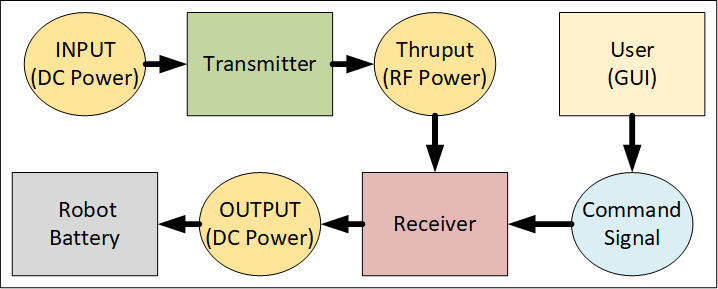
\includegraphics[width=0.84\linewidth]{black_box_power}
\caption{Operation Story Block Diagram}
\end{figure}
\hfill \\
\pagebreak
\section{Target Specifications and Ethical Considerations}


\begin{multicols}{2}

	% Wrap Table Example

%\begin{wraptable}[1]{2}[3]{4}
%...
%\end{wraptable}
%Number of lines (optional)
%“r” for right and “l” for left figure placement.
%Overhang (optional)
%Width to be reserved.


%\newcolumntype{C}{>{\centering\arraybackslash} m{6cm} }  %# New column type
%\newcolumntype{R}{>{\raggedleft \arraybackslash} m{6cm} }  %# New column type

\begin{wraptable}{l}{0.95\linewidth}
\centering
\caption{Receiver Specifications}
\begin{tabular} {| r | c | }
\hline
\parbox{0.45\linewidth}{\raggedleft \hfill \\ Charge time \\  (4Ah Battery Pack)\\} & 5 Hours Max\\
\hline
Battery pack voltage & 14.2 V  \\
\hline
\parbox{0.45\linewidth}{\raggedleft \hfill \\  Coupling Efficiency \\ Transmitter to Receiver\\[0.4em]} & 90\%\\
\hline
\parbox{0.45\linewidth}{\raggedleft \hfill \\  AC-DC \\ Conversion Efficiency} & 80\%\\
\hline
\parbox{0.45\linewidth}{\raggedleft \hfill \\  Charging Controller \\  DC-DC converter} & 85\%\\[0.4em]
\hline
\parbox{0.45\linewidth}{\raggedleft \hfill \\  Overall Receiver \\  Conversion Efficiency} & 61.2\%\\[0.4em]
\hline
\parbox{0.45\linewidth}{\raggedleft \hfill \\  Maximum Battery \\ Charging Current} &   \parbox{0.45\linewidth}{\centering 1.25 A (14.7 V \\ battery pack)}\\
\hline
\parbox{0.45\linewidth}{\raggedleft \hfill \\  Charger Subsystem \\  Charge Protocol} &  \parbox{0.45\linewidth}{\centering \hfill \\  Constant Current \\Constant Voltage \\(Li-ION Battery)}\\
\hline
Battery Type &   \parbox{0.45\linewidth}{\centering\hfill \\  Lithium-Ion \\ (4 x18650 in Series or 2P4S Configuration)}\\
\hline
\parbox{0.45\linewidth}{\raggedleft \hfill \\  Power Negotiation} &  \parbox{0.45\linewidth}{\centering\hfill \\ Bluetooth 5 LE\\}\\
\hline
\parbox{0.45\linewidth}{\raggedleft \hfill \\  Transmitter Locator \\ Method \\[0.4em]} &   \parbox{0.45\linewidth}{\centering \hfill \\  RF Localization  [Bluetooth]}\\
\hline
Deliverable Demo &   \parbox{0.45\linewidth}{\centering \hfill \\  Self-Moving Device (Robot)}\\
\hline
Telemetry &   \parbox{0.45\linewidth}{\centering \hfill \\  Report State \\to GUI Device}\\[0.4em]
\hline
LCD display &   \parbox{0.45\linewidth}{\centering \hfill \\  Diagnostic Character \\String Display}\\
\hline
\end{tabular}
\end{wraptable}
 
\vfill
\columnbreak
%%%%%%%%%%%%%%%%%%%%%%%%%%%%%

\begin{wraptable}{l}{0.95\linewidth}
\centering
\caption{Transmitter Specifications}
\begin{tabular} {| r | c | }
\hline
Operating frequency & 13.56 MHz\\
\hline
RF power output & 30 W\\
\hline
Max operating range & 30 cm\\
\hline
DC Power supply  & 12V 5A max.  \\
\hline
\parbox{0.45\linewidth}{\raggedleft  Conversion Efficiency\\ DC-AC\\[0.4em]}  & 80\%\\
\hline
Telemetry &\parbox{0.48\linewidth}{\centering Report State \\to GUI Device\\[0.4em]}\\
\hline
\end{tabular}
\end{wraptable}



\begin{wraptable}{l}{0.95\linewidth}
\centering
\caption{Communication Link Specifications}
\begin{tabular} {| r | c | }
\hline
\parbox{0.45\linewidth}{\raggedleft Communication Medium \\[0.4em]} &  \parbox{0.48\linewidth}{\centering Bluetooth 5 LE}\\
\hline
\parbox{0.45\linewidth}{\raggedleft Protocol} &  \parbox{0.48\linewidth}{\centering TBD}\\
\hline
\end{tabular}
\end{wraptable}


\begin{wraptable}{l}{0.95\linewidth}
\centering
\caption{GUI Specifications}
\begin{tabular} {| r | c | }
\hline
\parbox{0.45\linewidth}{\raggedleft GUI OS} & \parbox{0.48\linewidth}{\centering \hfill \\ WinOS, IOS, \\ Linux, \& Android}\\[0.4em]
\hline
\parbox{0.45\linewidth}{\raggedleft License} &    \parbox{0.48\linewidth}{\centering LGPL 3.0} \\
\hline
\parbox{0.45\linewidth}{\raggedleft Software Architecture} &   \parbox{0.48\linewidth}{\centering \hfill \\ Model-Controller-View (MCV) Architecture\\[0.4em]} \\
\hline
\parbox{0.45\linewidth}{\raggedleft Delivery Model} &   \parbox{0.48\linewidth}{\centering \hfill \\ Open Source \\ (Free App Download)} \\[0.4em]
\hline
%\parbox{0.45\linewidth}{\raggedleft Deployment Model} &   \parbox{0.45\linewidth}{\centering Open Source / Free To Download App} \\
%\hline
\end{tabular}
\end{wraptable}
 \hfill \\
 \vfill 

\end{multicols}

\section{Final Design Specifications}
\subsection{Feasibility Study}

\indent \indent
The design consists of two subsystems: the transmitter and the receiver. This product is expected to be used by hobbyists and prototype designers for different applications that require contactless charging. There is no similar device available in the price range from \$200 to \$400.  The expected cost of the charger system is \$300. There are some commercial chargers available right now and the cost of that system is \$2000. The price of \$300 per system will make wireless charging affordable for hobbyists and freelance hardware developers.\\

\indent
The design tools such as Altium designer and Multisim simulator are available free of charge to all group members using the provided UT Tyler license. Also, parts manufacturers are providing free simulation and evaluation tools for development. In addition to the software evaluation kits may be required for testing certain parts of the system such as the microcontroller, Bluetooth module, and the battery charger controller. Most of those evaluation modules are already purchased and they are available to team members. Evaluation kits are purchased by Indus instruments.\\

\indent
The system is designed such that it uses standard components that are available at any electronic components store and they can be purchased without restrictions. PCB fabrication will be given to a company located in China that is offering quick turnaround PCB fabrication and fast shipping. Components purchasing and printed circuit board assembly will be done at Indus Instruments. Indus Instruments have all the necessary equipment that can handle surface mount components.\\

\indent
All test equipment required for development and testing will be available. Indus Instruments will provide space and necessary test equipment for the wireless charging system prototype evaluation and testing.\\

\indent
The final product cost is estimated at around \$300 (for small quantities). Most likely for larger quantities, it is possible to decrease the cost even more. 

\subsection{Microcontroller}

\indent \indent
There are four aspects to analyze: economics, technical, legal, and scheduling. A single MSP430FR5994 part costs about \$3 to \$4, while the MSP-EXP430FR5994 LaunchPad kit costs \$16.99. Considering the team only needs two of these microcontrollers (one for the transmitter and one for the receiver), this is an economic and reasonable cost. \cite{MSP430FR599x}  \cite{testKit}. On the technical side, this microcontroller’s memory, voltage supply limitations, UART and I2Cmode specifications, and overall low power consumption makes it the ideal model for our project needs \cite{MSP430FR599x}. Some of the most important standards TI’s MSP430FR5994 complies with include ANSI, JEDEC, and ESDA \cite{MSP430FR599x}. Lastly, the team already has in hands the LaunchPad kit for the microcontroller. The individual microcontrollers are also ready-to-purchase items with delivery times of less than 7 days. More testing will be done once the team has the first PCB design in hands. 

\subsection{Transmitter Coil}

%%%%%%  COME BACK TO ME %%%%%%%%%%%%%%%%%%%%%%%%%%%%%%%%%%%%%%%%%%%%%%%%%%%%%%%%%%%%%%%%%%%%%%%%%%%%%%%%%%%%%%%%%%%%%%%%%%%%%%%%%%%%%%%%%%%%%%%%%%%%%%%%%%%%%%%%%%%%%%%%%%%%%%%%%%%%%%%%%%%%%%%%%%%%%%%%%%%%%%%%%%%%%%%%%%%%%%%%%%%%%%%%%%%%%%%%%%%%%%%%%%%%%%%%%%%%%%%%%%%%%%%%%%%%%%%%%%%%%%%%%%%%%%%%%%%%%%%%%%%%%%%%%%%%%%%%%%%%%%%%%%%%%%%%%%%%%%%%%%%%%%%%%%%%%%%%%%%%%%%%%%%%%%%%%%%%%%%%%%%%%%%%%%%%%%%%%%%%%%%%%%%%%%%%%%%%%%%%%%%%%%%%%%%%%%%%%%%%%%%%%%%%%%%%%%%%%%%%%%%%%%%%%%%%%%%%%%%%%%%%%%%%%%%%%%%%%%%%%%%%%%%%%%%%%%%%%%%%%%%%%%%%%%%%%%%%%%%%%%%%%%%%%%%%%%%%%%%%%%%%%%%%%%%%%%%%%%%%%%%%%%%%%%%%%%%%%%%%%%%%%%%%%%%%%%%%%%%%%%%%%%%%%%%%%%%%%%%%%%%%%%%%%%%%%%%%%%%%%%%%%%%%%%%%%%%%%%%%%%%%%%%%%%%%%%%

\indent \indent
The circular planar coil was the most inexpensive approach, the copper tubing to make the coils has an approximate value of  \$15.99. The design properties also significantly contributed to reducing the complexity of acquiring the main coil parameters. It was important to take this factor into account because of the time constraint of two months. In order to reduce the complexity in our project, the spiral planar design was the best option.\\

\indent
The calculation of the inductance formula in the planar spiral design was easier to acquire than the other two proposed solutions. This was crucial because it significantly gave the project a higher chance of matching the predestined inductance of the circuit requirement of .909 $\mu$H.\\

\indent
The economical and ethical considerations did not affect our decision making as much, due to the fact that there were not many differences. Furthermore, this design was appropriate for our project and the team does have the budget, resources and time to successfully to implement this design. \\

\indent
The planar spiral coil design allows the project to more reduces the complexity of the formulas implemented in the calculations. 

%%%%%%%%%%%%%%%%%%%%%%%%%%%%%%%%%%%%%%%%%%%%%%%%%%%%%%%%%%%%%%%%%%%%%%%%%%%%%%%%%%%%%%%%%%%%%%%%%%%%%%%%%%%%%%%%%%%%%%%%%%%%%%%%%%%%%%%%%%%%%%%%%%%%%%%%%%%%%%%%%%%%%%%%%%%%%%%%%%%%%%%%%%%%%%%%%%%%%%%%%%%%%%%%%%%%%%%%%%%%%%%%%%%%%%%%%%%%%%%%%%%%%%%%%%%%%%%%%%%%%%%%%%%%%%%%%%%%%%%%%%%%%%%%%%%%%%%%%%%%%%%%%%%%%%%%%%%%%%%%%%%%%%%%%%%%%%%%%%%%%%%%%%%%%%%%%%%%%%%%%%%%%%%%%%%%%%%%%%%%%%%%%%%%%%%%%%%%%%%%%%%%%%%%%%%%%%%%%%%%%%%%%%%%%%%%%%%%%%%%%%%%%%%%%%%%%%%%%%%%%%%%%%%%%%%%%%%%%%%%%%%%%%%%%%%%%%%%%%%%%%%%%%%%%%%%%%%%%%%%%%%%%%%%%%%%%%%%%%%%

\subsection{Transmitter}

\indent \indent
The transmitter class-E amplifier circuit was simulated at an efficiency of 98\%. The actual transmitter efficiency would be around 90\%. In the simulation, it was determined that the current required to power the class-E amplifier is 0.9 A at 30 V. The power for the transmitter will be supplied by using an external 48 V AC to DC converter followed by a step-down converter in the transmitter subsystem.\\

\indent
The main concern in this subsystem is the immunity of the supporting circuits to the RF electromagnetic field generated by the transmitter coil. The transmitter coil placement must be done such that the electromagnetic field has minimal effects on the electronic circuits in the transmitter. The transmitter sensitive electronic parts may require EMI shields.\\

\indent
During the simulation, the high voltage across the coil was observed. The highest voltage observed was 320 Vpp. That voltage poses a serious electric shock hazard. Therefore, the transmitter coil insulation must be capable of withstanding voltages that are in the 500V to 1kV range to provide a safety margin for the design. One way of achieving this is to make a plastic box that would contain the transmitter coil and have insulation that is capable of withstanding voltages in the 500 V to 1000 V range.  \\

\indent
Heat dissipation in the Class E amplifier circuit is expected to be around 3W (based on the efficiency of 90\%). That dissipation will occur in inductors, capacitors (due to ESR), and the amplifier transistor. The transistor will have a proper heatsink to prevent overheating. Since the dissipation in the transistor is very small (on-resistance is 50 mΩ) the proper thermal management will be achieved on the printed circuit board. Coils used in the transmitter will be designed such that the col resistance is minimized which also will decrease the heat dissipation in the transmitter circuit.

\subsection{Receiver}

\noindent \noindent
There is a possibility that the receiver RF to DC stage performs with higher losses than the losses that were determined in the simulation. According to the simulation data, the RF to DC conversion will be 81\% efficient. In the system specification, the conversion efficiency is set to 80\%. It is important to keep efficiency above 80\% to prevent excessive heat generation. If received power is 25W and efficiency is  80\% then power dissipation is 5 W.   \\

\indent
The excessive heat may have adverse effects on battery life and the speed of charging \cite{TPSM265R1}. A higher temperature environment requires lower charging currents to prevent further temperature rise and damage to the battery cells. Also, excessive heat generation must be minimized to avoid the use of fans and large heat-sinks. Heat-sinks and fans would increase the cost and the size of our product.   If during the prototype test phase efficiency drops below 80\% the circuit must be redesigned to achieve the target specification efficiency. \\

\indent
One problem that is likely to occur is the interference in the battery charging and communication link circuits caused by a strong electromagnetic field generated by the transmitter coil. Even though all good practices will be followed for the circuit board design the electromagnetic interference still may not be prevented. Charging circuit disruption can cause battery failure due to overcharging or overheating. If this problem occurs the additional EMI shielding will be required. The shielding includes placing metal boxes over sensitive electronic subcircuits and placing additional filters in series with DC power supplies for sensitive parts such as a microcontroller, Bluetooth module, and charger controller.

\pagebreak

\subsection{Thermal Considerations for 3.3V and 5V Voltage Regulators}

\indent \indent
According to the simulation data both parts have small power dissipation. The largest power dissipation is 0.18 W (5.0V regulator).\\

\indent
The graph below provides thermal resistance junction to ambient as a function of the printed circuit board. The equation below can be used to find the required thermal resistance junction to ambient ($\Theta_{JA}$). The estimated ambient temperature in the transmitter is 45$^{\circ}$C.

\begin{equation}
\Theta_{JA} = \frac{125^\circ C - T_{A(max)}}{P_{D(max)}} \Bigg[\frac{^\circ C}{W}\Bigg]
\end{equation}

\noindent
$\Theta_{JA}$ = $\frac{125-45}{0.18}$ = 444.44 \Big[$\frac{^\circ C}{W}$\Big]

\noindent
The estimated transmitter PCB area will be around 100cm2. Given the board size and thermal resistance vs. board size, those regulators will have a proper heatsink.

\begin{figure}[h!]
\centering
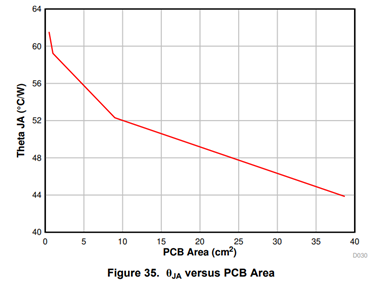
\includegraphics[width=0.9\linewidth]{pcb_JA_theta}
\caption{Thermal Resistance vs. PCB Area \cite{TPSM265R1}}
\end{figure}

\pagebreak

\noindent
Thermal considerations(for class E amplifier voltage regulator (30V, 1.0A buck converter) 

\begin{equation}
T_{A(max)} = T_{J(max)} - R_{TH} \cdot P_{TOT}
\end{equation}
\noindent
$\cdot $ P$_{TOT}$ is the total device power dissipation in [W]
\\
\noindent
$\cdot $ T$_A$ is the ambient temperature in [$^\circ$C]
\\
\noindent
$\cdot $ T$_J$ is the junction temperature in [$^\circ$C]
\\
\noindent
$\cdot $ R$_{TH}$ is the thermal resistance of the package \Big[$\frac{^\circ C}{W}$\Big]
\\
\noindent
$\cdot $ T$_{A(max)}$ is the maximum ambient temperature in [$^\circ$C]
\\
\noindent
$\cdot $ T$_{J(max)}$ is the maximum junction temperature in [$^\circ$C]
\\

\noindent
The expected ambient temperature is 40$^\circ$C (that is temperature inside the transmitter enclosure).\\
Thermal resistance for a standard board ($\Theta_{JA}$) is 62.5\Big[$\frac{^\circ C}{W}$\Big] \cite{TPS54160}.\\
From the simulation the total power dissipation is 1 W.\\
From the recommended operating conditions the maximum junction temperature is 150$^\circ$C \cite{TPS54160}.\\
Based on the data from the simulation and the datasheet the maximum ambient temperature can be determined\\
T$_{A(MAX)}$ = T$_{J(MAX)}$ - R$_{TH}$*P$_{TOT}$ \\
T$_{A(MAX)}$ = 150 – 62.5*1 = 87.5$^\circ$C\\
The expected ambient temperature is lower than the maximum temperature calculated based on simulation data. Therefore, this part will operate within specified recommended conditions in the datasheet.

\subsection{Charging Subsystem}

\indent \indent
The LTC4162-L is designed to manage a power path between an external input power source Vin, an output power V$_{out}$, and an installed battery pack. When external input power greater than the battery voltage is available at V$_{in}$, the LTC4162 will route V$_{in}$ to V$_{out}$ and charge the connected battery. If external power is interrupted or falls below V$_{bat}$, battery power will be automatically routed to V$_{out}$. As long as the battery has charge or a power source exists at V$_{in}$, V$_{out}$ will be supplied with power, but the voltage will range from V$_{bat}$ to V$_{in}$. In order to provide consistent voltage to the target device output power should be drawn directly from the battery. Leaving V$_{out}$ unused allows the maximum power point tracking feature to operate with optimal efficiency.\\

\indent
The LTC4162 draws power directly from Vout and has its own internal LDO linear regulators. All other components of the wireless receiver PCB must be powered by an appropriate DC-DC stage at V$_{out}$ that can convert any potential input voltage (i.e. 7.4-35 V) to the required operating voltages of 5 V and 3.3 V. These circuits will require power in order to operate and initiate charging. In the event that the battery is severely depleted and cannot power the microprocessor and Bluetooth interface, it will be necessary for the transmitter to be capable of initiating charging independently.\\

\indent
Since the LTC4162 has only an internal buck voltage regulator, the wireless power receiver subsystem must provide power to Vin that is higher than the voltage of the battery but below the maximum input voltage of 35V.\\

\indent
The LTC4162 approaches 95\% efficiency at recommended switching frequency when the input voltage is no more than approximately 5V above battery charging voltage, and surpasses 90\% in less ideal configurations. Heat losses will be in the range of three watts or less. It has a $\Theta_{JC}$ of 3.4 \Big[$\frac{^\circ C}{W}$\Big] and will be soldered to a four-layer PCB. The team does not anticipate any thermal management issues with this circuit.

\subsection{Battery Considerations}

Li-Ion batteries offer superb performance and high energy density, but require special attention to safety. Under normal circumstances the LTC4162-L will monitor battery voltage and avoid overcharging. A NTC thermistor will allow the LTC4162 to monitor local charging temperatures and limit current in accordance with JEIDA recommendations.\\

\indent
For safety reasons, the team requires stricter battery specifications than originally planned. While our charger’s thermistor can limit charging current in response to ambient temperature extremes, it cannot monitor individual cells--particularly if the battery pack is intended to be modular. While it can recognize and respond to abnormal battery voltages or short conditions, it cannot automatically determine maximum safe charging current. Any battery pack used must have a maximum charge current greater than the maximum current delivery of the charger. Battery packs must also meet UL1642 and IEC61960 standards and contain internal protection circuitry to limit charge and discharge currents and protect against thermal runaway.\\

\indent
The LTC4162 can deliver a maximum of 3.2 amps and has an efficiency of up to 95\%. Assuming optimal efficiency and 26 W output from the wireless receiver, the charging voltage must be at least $frac{25 W}{3.2 A}$ = 7.8 V in order to fully utilize the available power. Since the voltage of a typical Li-Ion cell is 3.7 V and the charging voltage is 4.2 V, the target battery pack should consist of two or more cells in series. The LTC4162 supports 1 to 8 cell series arrangements provided the input voltage is adequate. Optimal arrangements would include a 7.4V pack rated for 3.2 A charging, a 11.1 V pack rated for 2.2 A charging, or a 14.8 V pack rated for 1.7 A charging. The number of cells is set by selection pins and may be configured by a DIP switch or jumpers. It is not necessary to specify a specific number of cells for suitable battery packs, provided that they meet UL1642 and IEC61960 standards. The optimal balance of safe charging rates and performance will likely be found with packs utilizing six to eight 18650 cells or the equivalent. The power delivery estimates above are optimistic and actual power delivery from the charger may not reach these levels. As prototyping progresses, it will be possible to refine battery recommendations and expected charging times.\\

\pagebreak

\indent
Ideally, up to 25 W will be delivered to the battery pack, making the battery the largest potential source of heat in our system. Since the battery pack is intended to be a modular, removable component with flexible specifications, it will not necessary for it to be enclosed with the wireless receiver PCB and receiving coil. It will be connected by an appropriate low-loss cable and connector, and exact placement will be determined by the user application. For this reason, the team has specified that only battery packs with internal temperature monitoring and protection circuitry should be used with this charger.\\

\indent
Our original specifications suggested that the charging subsystem would be capable of detailed monitoring of battery health and charge state. The team has learned that this type of information must be obtained at the individual cell level by a specialized controller which is usually integrated into the battery pack itself. Our charge subsystem can only recognize an approaching low-battery condition by a drop in voltage, and cannot estimate battery capacity except by calculation using charging voltage, charge times and currents, and such data would be of limited use considering battery aging and user-replaceability. It will be possible to notify the user and target device of a drop in battery voltage, but more detailed fuel gauge and battery health information will require an SMBus enabled smart battery. An I2C line on the MSP430FR5994 will be reserved for communication with an optional SMBus capable smart battery pack. If feasible, optional battery pack telemetry may be polled by firmware and reported to the user along with the data already available from the LTC4162.\\

\indent
All the parts and design resources needed to complete the charging and power subsystem are readily available. Constructing this subsystem within the projected time-frame is feasible.

\begin{table}[h!]
\centering
\caption{Final Design's Charging Subsystem  Specifications}
\begin{tabular} {| r | c | }
\hline
\parbox{0.3\linewidth}{\raggedleft DC-DC stage from wireless receiver to V$_{in}$} &   \parbox{0.65\linewidth}{\hfill \\
May not be necessary, pending further determination of wireless receiver output voltage}\\
\hline
\parbox{0.3\linewidth}{\raggedleft DC-DC stage from V$_{out}$} &   \parbox{0.65\linewidth}{\hfill \\
5V at 100mA; 3.3V at 100 mA}\\
\hline
\parbox{0.3\linewidth}{\raggedleft Battery Requirements} &   \parbox{0.65\linewidth}{\hfill \\
UL1642 and IEC61960 compliant Li-Ion packs with 7.4-15 V$_{DC}$ nominal output voltage}\\
\hline
\parbox{0.3\linewidth}{\raggedleft \vspace{0.4em} Maximum Charging Current} &   \parbox{0.65\linewidth}{\hfill \\
3.2A (7.4V); 2.2A (11.1V); 1.7A (14.8V)}\\
\hline
\parbox{0.3\linewidth}{\raggedleft \vspace{0.4em} Provision for optional smart battery health and fuel gauge monitoring} &   \parbox{0.65\linewidth}{\hfill \\
Reserved I2C line from MSP430FR5994 with buffering}\\
\hline
\end{tabular}
\end{table}
\hfill \\

\subsection{Microcontroller Considerations}

\indent \indent
The MSP430FR5994 has a body size that ranges from 6mm by 6mm to 12mm by 12mm depending on the package the group purchases, 8KB RAM, 68 GPIO pins, 4 I$^2$C, 4 UART, up to four serial communication ports, and 20 ADC channels. The MSP430 series include limitations that range from safety to performance \cite{MSP430FR599x}.\\

\noindent
Relevant limitations to the project include:\\

\noindent
1. ESD (Electrostatic discharge) ratings. For a human-body model, safe discharge ratings are around 500 V to 1000 V, while for a charged-device model, safe discharge ratings are around 250 V. These regulations are taken from JEDEC JS-001 and JESD22-C101 respectively \cite{MSP430FR599x}.\\

\noindent
2. Absolute maximum ratings: voltage applied to any pin must be within -0.3 V to 4.1 V, voltage difference between DVCC and AVCC pins must stay within -0.3 V to 0.3 V (if not, writing errors could occur to RAM and FRAM), and current at any device pin must have a maximum of  -2 to 2 mA \cite{MSP430FR599x}.\\

\noindent
3. Supply voltage applied should be within 1.8 V to 3.6 V, maximum ACLK frequency should be 50 kHz, and maximum SMCLK frequency should be 16 MHz \cite{MSP430FR599x}.\\

\noindent
4. For the eUSCI I$^2$C, eUSCI (enhanced universal serial communication interface) input clock frequency should not exceed 16 MHz, SCL clock frequency should not exceed 400 kHz \cite{MSP430FR599x}.


\subsection{Firmware Requirements: Transmitter}

\indent \indent
The Wireless Power Transmission Stage (Transmitter) will be controlled by an MSP430FR5994 running custom firmware. The firmware must meet the following requirements:\\

\noindent
1.) Activate or deactivate wireless transmitter.\\

\noindent
2.) Respond to commands received from a Bluetooth link with the Wireless Power Receiver Stage (Receiver), which may include requests for power delivery measurements or instructions to initiate or cease charging.\\

\noindent
3.) Continuously monitor wireless power transmitter current and voltage and calculate delivered power.\\

\noindent
4.) Automatically cease power transmission when the Receiver requests a shutdown or if severe interference is detected.\\

\noindent
5.) Communicate operating status to the Receiver via Bluetooth, and directly to the user via fault LED’s or an installed LCD.


\subsection{Firmware Requirements: Receiver}

\indent \indent
The Wireless Power Receiver Stage (Receiver) will be controlled by an MSP430FR5994 running custom firmware. The firmware must meet the following requirements:\\

\noindent
1.) Link to the Transmitter over Bluetooth.\\

\noindent
2.) Link to user GUI device over Bluetooth.\\

\noindent
3.) Link to an optional UART connection with the target device.\\

\noindent
4.) Respond to queries or instructions from the Bluetooth connection to the user GUI or from the optional UART connection.\\

\noindent
5.) Monitor charging state and battery status though I2C connection with LTC4162 and optional SMBus link with smart battery.\\

\noindent
6.) Recognize low voltage state or optional low capacity battery warning and notify the user and target device.\\

\noindent
7.) Signal the Transmitter via Bluetooth to initiate charging when instructed by the user or target device.\\

\noindent
8.) Continuously monitor wireless power receiver current and voltage and calculate delivered power.\\

\noindent
9.) Monitor reported power transmission from the Transmitter, compare it with received power, and recognize excessive power losses that could indicate unsafe interference conditions\\

\noindent
10.) In the event of excessive transmission losses, instruct the Transmitter to cease power transmission. Notify the user and target device of the error condition.\\

\indent
The Transmitter and Receiver firmware will be developed with Texas Instruments Code Composer Studio. The team has suitable Launchpad development boards and access to all necessary documentation and libraries are available. The team is composed of multiple experienced programmers in our group. The firmware requirements are limited and well-defined and completing it within our scheduled time-frame is feasible.

\pagebreak

\subsection{Software Requirements: GUI}

The GUI will be operated on multiple platforms and rely upon QT5 to operate.  The software must fulfill the following requirements:\\

\noindent
1.) Provide connection to transmitter and receiver for the product's user that grants sufficient control over the product's hardware\\

\noindent
2.) Serve as a platform for custom messages to and from the user's device connected to the receiver.\\

\noindent
3.) Provide alert system via push notifications and continuous monitoring of the transmitter and receiver.\\


\subsection{Coil Considerations}

\begin{table}[h!]
\centering
\caption{Final Design's Coil Tubing Specifications}
\begin{tabular} {| r | c | }
\hline
\parbox{0.3\linewidth}{\raggedleft
Material
} &   \parbox{0.45\linewidth}{\hfill \\
122 Copper
}\\
\hline
\parbox{0.3\linewidth}{\raggedleft
Tube Size
} &   \parbox{0.45\linewidth}{\hfill \\
$\frac{1}{8}$ [in]
}\\
\hline
\parbox{0.3\linewidth}{\raggedleft
Outter Diameter (OD)
} &   \parbox{0.45\linewidth}{\hfill \\
$\frac{1}{4}$ [in]
}\\
\hline
\parbox{0.3\linewidth}{\raggedleft
Wall Thickness
} &   \parbox{0.45\linewidth}{\hfill \\
0.049 [in]
}\\
\hline
\parbox{0.3\linewidth}{\raggedleft
Inner Diameter (ID)
} &   \parbox{0.45\linewidth}{\hfill \\
0.152 [in]
}\\
\hline
\parbox{0.3\linewidth}{\raggedleft
Fabrication
} &   \parbox{0.45\linewidth}{\hfill \\
Seamless
}\\
\hline
\parbox{0.3\linewidth}{\raggedleft
Bending Method
} &   \parbox{0.45\linewidth}{\hfill \\
By hand
}\\
\hline
\parbox{0.3\linewidth}{\raggedleft
Temper Rating
} &   \parbox{0.45\linewidth}{\hfill \\
Soft
}\\
\hline
\parbox{0.3\linewidth}{\raggedleft
Compatible Tube Fittings
} &   \parbox{0.45\linewidth}{\hfill \\
Compression, Solder Connect
}\\
\hline
\parbox{0.3\linewidth}{\raggedleft
Specifications met
} &   \parbox{0.45\linewidth}{\hfill \\
ASTM B75\\
RoHS 3(2015/863/EU) Compliant
}\\
\hline
\parbox{0.3\linewidth}{\raggedleft
Resistivity 
} &   \parbox{0.45\linewidth}{\hfill \\
1.68 x 10$^{-8}$ [$\Omega$/m]
}\\
\hline
\parbox{0.3\linewidth}{\raggedleft
Conductivity 
} &   \parbox{0.45\linewidth}{\hfill \\
5.96 x 10$^7$ [S/m]
}\\
%\hline
%\parbox{0.3\linewidth}{\raggedleft
%
%} &   \parbox{0.45\linewidth}{\hfill \\
%
%}\\
\hline
\end{tabular}
\end{table}
\hfill \\

\indent
This tubing has good corrosion resistance and excellent heat transfer qualities. All tubing meets international standards for copper tubing. Important to note: Tube size is an accepted industry designation, not an actual size  \cite{rfCond}.

\begin{table}[h!]
\centering
\caption{Final Design's Receiver Coil Specifications}
\begin{tabular} {| r | c | }
\hline
\parbox{0.3\linewidth}{\raggedleft
Outside Diameter of Coils (Do) 
} &   \parbox{0.45\linewidth}{\hfill \\
90 mm
}\\
\hline
\parbox{0.3\linewidth}{\raggedleft
 Number of Turns 
} &   \parbox{0.45\linewidth}{\hfill \\
4
}\\
\hline
\parbox{0.3\linewidth}{\raggedleft
Length
} &   \parbox{0.45\linewidth}{\hfill \\
729.6 mm
}\\
\hline
\parbox{0.3\linewidth}{\raggedleft
Spacing
} &   \parbox{0.45\linewidth}{\hfill \\
4.81 mm
}\\
\hline
\parbox{0.3\linewidth}{\raggedleft
Width of Tubing
} &   \parbox{0.45\linewidth}{\hfill \\
3.175 mm
}\\
\hline
\parbox{0.3\linewidth}{\raggedleft
Inner Diameter (Di) 
} &   \parbox{0.45\linewidth}{\hfill \\
26.12 mm
}\\
\hline
\parbox{0.3\linewidth}{\raggedleft
Winding Radius 
} &   \parbox{0.45\linewidth}{\hfill \\
29.03 mm
}\\
\hline
\parbox{0.3\linewidth}{\raggedleft
Radial Depth 
} &   \parbox{0.45\linewidth}{\hfill \\
31.94 mm
}\\
\hline
\parbox{0.3\linewidth}{\raggedleft
Inductance
} &   \parbox{0.45\linewidth}{\hfill \\
909.66 nH.
}\\
\hline
\parbox{0.3\linewidth}{\raggedleft
Capacitance
} &   \parbox{0.45\linewidth}{\hfill \\
150.55 pF
}\\
\hline
\parbox{0.3\linewidth}{\raggedleft
Frequency
} &   \parbox{0.45\linewidth}{\hfill \\
13.6 MHz
}\\
\hline
\parbox{0.3\linewidth}{\raggedleft
Resistance (Dc) 
} &   \parbox{0.45\linewidth}{\hfill \\
1.5462 m$\Omega$
}\\
\hline
\parbox{0.3\linewidth}{\raggedleft
Total Resistance 
} &   \parbox{0.45\linewidth}{\hfill \\
69.46 m$\Omega$
}\\
\hline
\parbox{0.3\linewidth}{\raggedleft
Quality Factor 
} &   \parbox{0.45\linewidth}{\hfill \\
1119.09
}\\
\hline
%\parbox{0.3\linewidth}{\raggedleft
%
%} &   \parbox{0.45\linewidth}{\hfill \\
%
%}\\
%\hline
\end{tabular}
\end{table}
\hfill \\

\pagebreak
\hfill \\
\pagebreak

\subsection{Specification Summary}

\begin{table}[h!]
\centering
\caption{Final Design's Receiver Specifications}
\begin{tabular} {| r | c | }
\hline
\parbox{0.3\linewidth}{\raggedleft
Charge time(4Ah Battery Pack)
} &   \parbox{0.65\linewidth}{\hfill \\
5 Hours Max
}\\
\hline
\parbox{0.3\linewidth}{\raggedleft
Battery pack voltage
} &   \parbox{0.65\linewidth}{\hfill \\
User Selectable: 7.4V-14.2 V
}\\
\hline
\parbox{0.3\linewidth}{\raggedleft
Coupling Efficiency Transmitter to Receiver %\vspace{0.2em}		%%% 			<---- 		THIS WORKS				%%%
} &   \parbox{0.65\linewidth}{\hfill \\
90\%
}\\
\hline
\parbox{0.3\linewidth}{\raggedleft
AC-DC Conversion Efficiency
} &   \parbox{0.65\linewidth}{\hfill \\
80\% 
}\\
\hline
\parbox{0.3\linewidth}{\raggedleft
Charging Controller DC-DC Converter
} &   \parbox{0.65\linewidth}{\hfill \\
85\%
}\\
\hline
\parbox{0.3\linewidth}{\raggedleft
Overall Receiver Conversion Efficiency
} &   \parbox{0.65\linewidth}{\hfill \\
61.2\%
}\\
\hline
\parbox{0.3\linewidth}{\raggedleft
Battery Requirements:
} &   \parbox{0.65\linewidth}{\hfill \\
UL1642 and IEC61960 compliant Li-ion packs.
}\\
\hline
\parbox{0.3\linewidth}{\raggedleft
Maximum Battery Charging Current
} &   \parbox{0.65\linewidth}{\hfill \\
3.2A (7.4V); 2.2A (11.1V); 1.7A (14.8V)
}\\
\hline
\parbox{0.3\linewidth}{\raggedleft
Charger Subsystem Charge Protocol
} &   \parbox{0.65\linewidth}{\hfill \\
Constant Current Constant Voltage (Li-Ion Battery)
}\\
\hline
\parbox{0.3\linewidth}{\raggedleft
Battery Type 
} &   \parbox{0.65\linewidth}{\hfill \\
UL1642 and IEC61960 compliant Li-Ion packs; 7.4-15 VDC nominal output voltage.
}\\
\hline
\parbox{0.3\linewidth}{\raggedleft
Power Negotiation
} &   \parbox{0.65\linewidth}{\hfill \\
Using Bluetooth 5 LE
}\\
\hline
\parbox{0.3\linewidth}{\raggedleft
Deliverables
} &   \parbox{0.65\linewidth}{\hfill \\
Wireless resonant charger with approximately 30W power transmission capability.\\
Stretch Goal: a mobile device to demonstrate autonomous charging.
}\\
\hline
\parbox{0.3\linewidth}{\raggedleft
Telemetry
} &   \parbox{0.65\linewidth}{\hfill \\
Report State to GUI Device
}\\
\hline
\parbox{0.3\linewidth}{\raggedleft
LCD display
} &   \parbox{0.65\linewidth}{\hfill \\
Diagnostic Data\\
Character String Display
}\\
\hline
%\parbox{0.3\linewidth}{\raggedleft
%
%} &   \parbox{0.65\linewidth}{\hfill \\
%
%}\\
%\hline
\end{tabular}
\end{table}
\hfill \\


\begin{table}[h!]
\centering
\caption{Final Design's Transmitter Specifications}
\begin{tabular} {| r | c | }
\hline
\parbox{0.3\linewidth}{\raggedleft
Operating Frequency
} &   \parbox{0.65\linewidth}{\hfill \\
13.56 MHz
}\\
\hline
\parbox{0.3\linewidth}{\raggedleft
RF Power Output
} &   \parbox{0.65\linewidth}{\hfill \\
30 W
}\\
\hline
\parbox{0.3\linewidth}{\raggedleft
Max. Charging Distance
} &   \parbox{0.65\linewidth}{\hfill \\
30 cm
}\\
\hline
\parbox{0.3\linewidth}{\raggedleft
DC Power supply
} &   \parbox{0.65\linewidth}{\hfill \\
48V 1.25A min.
}\\
\hline
\parbox{0.3\linewidth}{\raggedleft
Conversion Efficiency DC-AC
} &   \parbox{0.65\linewidth}{\hfill \\
80\%
}\\
\hline
\parbox{0.3\linewidth}{\raggedleft
Telemetry
} &   \parbox{0.65\linewidth}{\hfill \\
Report State to Receiver
}\\
\hline
%\parbox{0.3\linewidth}{\raggedleft
%
%} &   \parbox{0.45\linewidth}{\hfill \\
%
%}\\
%\hline
\end{tabular}
\end{table}
\hfill \\


\begin{table}[h!]
\centering
\caption{Final Design's Communication Link Specifications}
\begin{tabular} {| r | c | }
\hline
\parbox{0.3\linewidth}{\raggedleft
 Communication Medium
} &   \parbox{0.65\linewidth}{\hfill \\
Bluetooth 5 LE
}\\
\hline
\parbox{0.3\linewidth}{\raggedleft
Protocols
} &   \parbox{0.65\linewidth}{\hfill \\
GUI: Host Controller Interface (HCI)\\
Receiver-\>transmitter: Synchronous Connection-Oriented (SCO) link
}\\
\hline
%\parbox{0.3\linewidth}{\raggedleft
%
%} &   \parbox{0.45\linewidth}{\hfill \\
%
%}\\
%\hline
\end{tabular}
\end{table}
\hfill \\


\begin{table}[h!]
\centering
\caption{Final Design's GUI Specifications}
\begin{tabular} {| r | c | }
\hline
\parbox{0.3\linewidth}{\raggedleft
OS
} &   \parbox{0.65\linewidth}{\hfill \\
WinOS, IOS, Linux, \& Android
}\\
\hline
\parbox{0.3\linewidth}{\raggedleft
License
} &   \parbox{0.65\linewidth}{\hfill \\
 LGPL 3.0
}\\
\hline
\parbox{0.3\linewidth}{\raggedleft
Software Architecture
} &   \parbox{0.65\linewidth}{\hfill \\
Model-Controller-View (MCV) Architecture
}\\
\hline
\hline
\parbox{0.3\linewidth}{\raggedleft
Delivery Model 
} &   \parbox{0.65\linewidth}{\hfill \\
Open Source\\
Free App Download
}\\
\hline
%\parbox{0.3\linewidth}{\raggedleft
%
%} &   \parbox{0.45\linewidth}{\hfill \\
%
%}\\
%\hline
\end{tabular}
\end{table}
\hfill \\
\begin{table}[h!]
\centering
\caption{Ethical and Professional Considerations}
\begin{tabular} {| r | c | }
\hline
\parbox{0.3\linewidth}{\raggedleft Public Health} &   \parbox{0.65\linewidth}{\hfill \\
$\cdot$ Medical Equipment RF Exposure \\ $\cdot$ Electrical Shock \\ $\cdot$ Chemical Exposure}\\
\hline
\parbox{0.3\linewidth}{\raggedleft Safety and Wellness} &   \parbox{0.65\linewidth}{\hfill \\
$\cdot$ RF Bandwidth Jamming \\ $\cdot$ Electrical Shock \\ $\cdot$ Chemical Exposure}\\
\hline
\parbox{0.3\linewidth}{\raggedleft Global Factors} &   \parbox{0.65\linewidth}{\hfill \\
$\cdot$ International Governing Bodies \\ $\cdot$ Sourcing Restrictions \\ $\cdot$ Inter-Market Penetrability}\\
\hline
\parbox{0.3\linewidth}{\raggedleft Societal Factors} &   \parbox{0.65\linewidth}{\hfill \\
$\cdot$ Open-Source Capitalization\\ $\cdot$ STEM Educational Resources \\ $\cdot$ Professional Organizations \\ $\cdot$ Customer Privacy \& Security}\\
\hline
\parbox{0.3\linewidth}{\raggedleft Environmental Factors} &   \parbox{0.65\linewidth}{\hfill \\
$\cdot$ Chemical Pollution\\ $\cdot$ User Environmental Awareness\\ $\cdot$ Emergency Shut Off Cases}\\
\hline
\parbox{0.3\linewidth}{\raggedleft Economic Factors} &   \parbox{0.65\linewidth}{\hfill \\
$\cdot$ Open-Source Capitalization\\ $\cdot$ Specialty Clientele\\ $\cdot$ Rapid Agile-Deployment\\ $\cdot$ Light-Weight Production}\\
\hline
\end{tabular}
\end{table}
\hfill \\





%\pagebreak

\section{References}

\section*{Software References}

Block diagrams were rendered in Windows Visio Standard 2019.\\
Multisim circuits simulated in NI Multisim V.14.2 2019.\\
%% Need it include TI-TINA simulation software.\\

	%%%%%%%%%%%%%%%%%%%%%%%%%%%%%%%%%%%%%%%%%%
	%														 %
	%														 %
	%				Special Note on Print Bibliiography w/ .bib file				 %
	%														 %
	%	   \printbibliography[keyword={a},keyword={b}] --> keyword a AND keyword b 	 %
	%			\defbibfilter{example}{keyword={a} or keyword={b}}	 		 %
	%		   \printbibliography[filter=example] --> keyword a OR keyword b 			 %
	%														 %
	%														 %
	%%%%%%%%%%%%%%%%%%%%%%%%%%%%%%%%%%%%%%%%%%

\printbibliography[keyword={regulation},title={Regulatory References}]

\defbibfilter{DesignReference}{keyword={documentation} or keyword={design}}
\pagebreak
\printbibliography[filter=DesignReference,title={Design References}]

\printbibliography[keyword={catelog},title={Catelogs for Parts Investigated}]


%\pagebreak

%%%% 	Setting Configuration for Sections on Table of Contents and Pages 	%%%%%

\addappheadtotoc

\setcounter{section}{0}

% In Line
\titleformat{\section}{\normalfont\filcenter}{APPENDIX \Alph{section}:}{1em}{\MakeUppercase} 
\titleformat{\subsection}{\normalfont\itshape}{\arabic{subsection}.}{1em}{}

% Table of Contents
%\renewcommand{\thesection}{\Alph{section}}
\renewcommand{\thesubsection}{\thesection.\arabic{subsection}}

%\cftsetindents{section}{1em}{10em}

%%%% 	Sections on Table of Contents and Pages Configured 	%%%%%



%\pagebreak



	%%%%%%%%%%%%%%%%%%%%%%%%%%%%%%%%%%%%%%%%%%
	%														 %
	%														 %
	%		\pagenumbering{gobble}	"gobbles" or removes the pagination of the page  	 %
	%					and the following pages.						 %
	%														 %
	%		\pagenumbering{num_style}	sets the pagination of the page and 	  	 %
	%						the following pages						 %
	%														 %
	%						{num_style} List:						 %
	%														 %
	%				{roman} -> lowercase roman numerals           				 %
	%				{Roman} -> uppercase roman numerals           				 %
	%				{alph} -> lowercase alphabetical numerals           			 %
	%				{Alph} -> uppercase alphabetical numerals           			 %
	%				{arabic} -> standard decimal numerals (0-9)           			 %
	%														 %
	%			Altering \pagenumbering{} will restart the pagination at 1.			 %
	%			     See other tutorial for greater control of paginations.			 %
	%														 %
	%														 %
	%%%%%%%%%%%%%%%%%%%%%%%%%%%%%%%%%%%%%%%%%%




	%%%%%%%%%%%%%%%%%%%%%%%%%%%%%%%%%%%%%%%%%%
	%														 %
	%														 %
	%					Special Note on Quotation Marks					 %
	%														 %
	%			   Standard Quotation Mark (") --> right quotation mark			 %
	%			Double Reverse Accent Mark (``) --> left quotation mark	 		 %
	%			left quotation mark = \textquotedblleft vs \textquotedblright 		 %
	%														 %
	%														 %
	%%%%%%%%%%%%%%%%%%%%%%%%%%%%%%%%%%%%%%%%%%



	%%%%%%%%%%%%%%%%%%%%%%%%%%%%%%%%%%%%%%%%%%
	%														 %
	%														 %
	%					Special Note on Tables						 %
	%														 %
	%				   l = left, c = center, r = right alignment				 %
	%			   | in tabular sets borders between alignment sets		 		 %
	%	      \hline places a horizontal line across width of table above current the line  		 %
	%			   \\ (the endline command) begins next line of table.		 		 %
	%														 %
	%														 %
	%%%%%%%%%%%%%%%%%%%%%%%%%%%%%%%%%%%%%%%%%%


\end{document}




%%%%%%%%%%%%%%%%%%%%%%%%%%%%%%%%%%%%%%%%%%%%%%%%%%%%%%
%					 													  %
%					 													  %
%					  ALWAYS END THE DOCUMENT WITH								  %
%					 													  %
%							\end{document}									  %
%					 													  %
%					 													  %
%%%%%%%%%%%%%%%%%%%%%%%%%%%%%%%%%%%%%%%%%%%%%%%%%%%%%%